
%<*named>
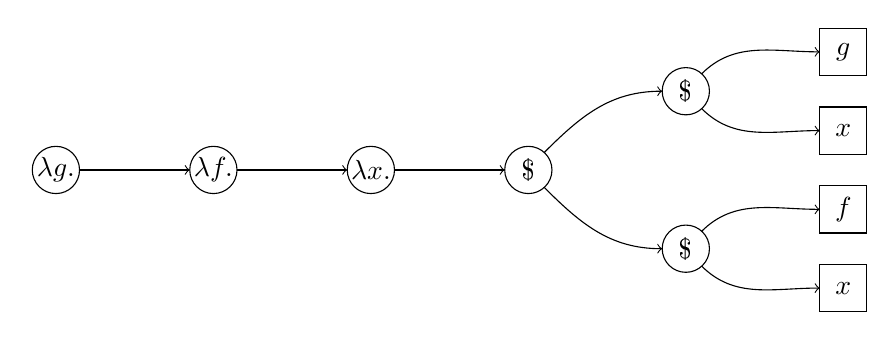
\begin{tikzpicture}
\draw (0,0) circle (.3cm) node[align=center] {$\lambda{}g.$};
\draw (2,0) circle (.3cm) node[align=center] {$\lambda{}f.$};
\draw (4,0) circle (.3cm) node[align=center] {$\lambda{}x.$};

\draw (6,0) circle (.3cm) node[align=center] {\$};

\draw (8,1) circle (.3cm) node[align=center] {\$};
\draw (10,1.5) node[align=center] {$g$} +(-.3cm,-.3cm) rectangle +(.3cm,.3cm);
\draw (10,.5)  node[align=center] {$x$} +(-.3cm,-.3cm) rectangle +(.3cm,.3cm);

\draw (8,-1) circle (.3cm) node[align=center] {\$};
\draw (10,-.5)  node[align=center] {$f$} +(-.3cm,-.3cm) rectangle +(.3cm,.3cm);
\draw (10,-1.5) node[align=center] {$x$} +(-.3cm,-.3cm) rectangle +(.3cm,.3cm);

\draw [->] (0.3,0)     to [out=0,in=180]   (1.7,0);
\draw [->] (2.3,0)     to [out=0,in=180]   (3.7,0);
\draw [->] (4.3,0)     to [out=0,in=180]   (5.7,0);
\draw [->] (6.2,-.22)  to [out=-45,in=180]  (7.7,-1);
\draw [->] (6.2,.22)   to [out=45,in=180]  (7.7,1);
\draw [->] (8.2,1.22)  to [out=45,in=180]  (9.7,1.5);
\draw [->] (8.2,.78)   to [out=-45,in=180] (9.7,.5);
\draw [->] (8.2,-1.22) to [out=-45,in=180] (9.7,-1.5);
\draw [->] (8.2,-.78)  to [out=45,in=180]  (9.7,-.5);
\end{tikzpicture}
%</named>

%<*debruijn>
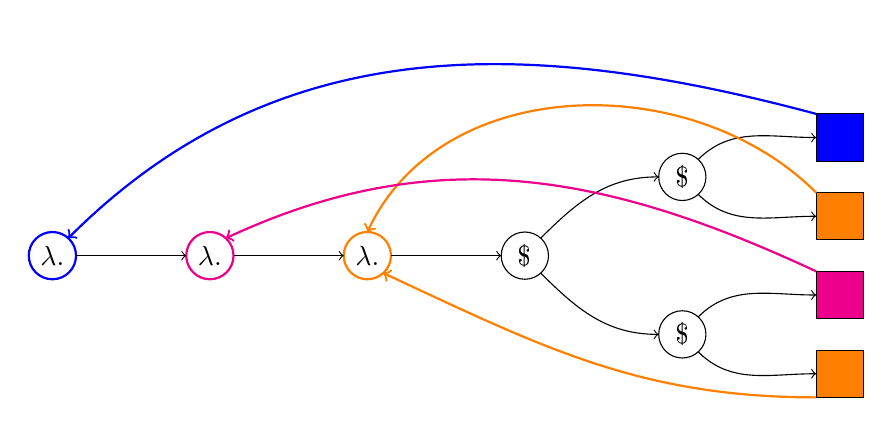
\begin{tikzpicture}
\draw[draw=blue   ,thick] (0,0) circle (.3cm) node[align=center] {$\lambda{}.$};
\draw[draw=magenta,thick] (2,0) circle (.3cm) node[align=center] {$\lambda{}.$};
\draw[draw=orange ,thick] (4,0) circle (.3cm) node[align=center] {$\lambda{}.$};

\draw (6,0) circle (.3cm) node[align=center] {\$};

\draw (8,1) circle (.3cm) node[align=center] {\$};
\draw[fill=blue]   (10,1.5) +(-.3cm,-.3cm) rectangle +(.3cm,.3cm);
\draw[fill=orange] (10,.5)  +(-.3cm,-.3cm) rectangle +(.3cm,.3cm);

\draw (8,-1) circle (.3cm) node[align=center] {\$};
\draw[fill=magenta] (10,-.5)  +(-.3cm,-.3cm) rectangle +(.3cm,.3cm);
\draw[fill=orange]  (10,-1.5) +(-.3cm,-.3cm) rectangle +(.3cm,.3cm);

\draw [->] (0.3,0)     to [out=0,in=180]   (1.7,0);
\draw [->] (2.3,0)     to [out=0,in=180]   (3.7,0);
\draw [->] (4.3,0)     to [out=0,in=180]   (5.7,0);
\draw [->] (6.2,-.22)  to [out=-45,in=180]  (7.7,-1);
\draw [->] (6.2,.22)   to [out=45,in=180]  (7.7,1);
\draw [->] (8.2,1.22)  to [out=45,in=180]  (9.7,1.5);
\draw [->] (8.2,.78)   to [out=-45,in=180] (9.7,.5);
\draw [->] (8.2,-1.22) to [out=-45,in=180] (9.7,-1.5);
\draw [->] (8.2,-.78)  to [out=45,in=180]  (9.7,-.5);

\draw[blue, thick] [->] (9.7,1.8)   to [out=165,in=45] (0.2,.22);

\draw[orange, thick] [->] (9.7,.8)   to [out=135,in=65] (4,.3);

\draw[magenta, thick] [->] (9.7,-.2)   to [out=155,in=25] (2.2,.22);

\draw[orange, thick] [->] (9.7,-1.8) to [out=180,in=335] (4.2,-.22);

\end{tikzpicture}
%</debruijn>

%<*codebruijn>
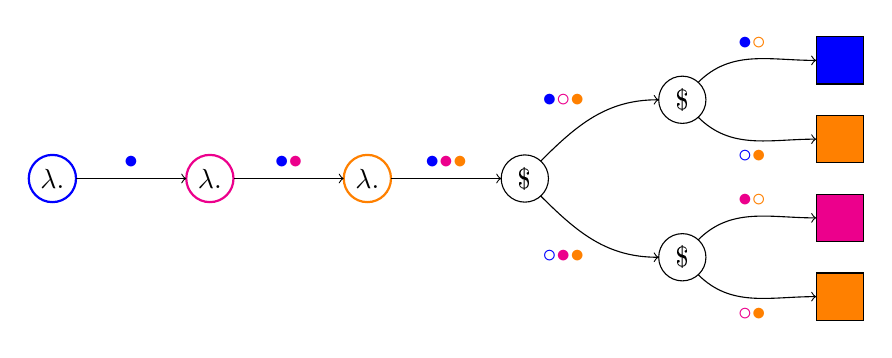
\begin{tikzpicture}
\draw[draw=blue   ,thick] (0,0) circle (.3cm) node[align=center] {$\lambda{}.$};
\draw[draw=magenta,thick] (2,0) circle (.3cm) node[align=center] {$\lambda{}.$};
\draw[draw=orange ,thick] (4,0) circle (.3cm) node[align=center] {$\lambda{}.$};

\draw (6,0) circle (.3cm) node[align=center] {\$};

\draw (8,1)    circle (.3cm) node[align=center] {\$};
\draw[fill=blue]   (10,1.5) +(-.3cm,-.3cm) rectangle +(.3cm,.3cm);
\draw[fill=orange] (10,.5)  +(-.3cm,-.3cm) rectangle +(.3cm,.3cm);

\draw (8,-1)    circle (.3cm) node[align=center] {\$};
\draw[fill=magenta] (10,-.5)  +(-.3cm,-.3cm) rectangle +(.3cm,.3cm);
\draw[fill=orange]  (10,-1.5) +(-.3cm,-.3cm) rectangle +(.3cm,.3cm);


\draw [->] (0.3,0)   to [out=0,in=180] node[above]{$\color{blue}{\bullet}$} (1.7,0);
\draw [->] (2.3,0)   to [out=0,in=180] node[above]{$\color{blue}{\bullet}\color{magenta}{\bullet}$} (3.7,0);
\draw [->] (4.3,0)   to [out=0,in=180] node[above]{$\color{blue}{\bullet}\color{magenta}{\bullet}\color{orange}{\bullet}$} (5.7,0);

\draw [->] (6.2,-.22)  to [out=-45,in=180] node[below left]{$\color{blue}{\circ}\color{magenta}{\bullet}\color{orange}{\bullet}$} (7.7,-1);
\draw [->] (6.2,.22)   to [out=45,in=180] node[above left]{$\color{blue}{\bullet}\color{magenta}{\circ}\color{orange}{\bullet}$} (7.7,1);
\draw [->] (8.2,1.22)  to [out=45,in=180] node[above]{$\color{blue}{\bullet}\color{orange}{\circ}$} (9.7,1.5);
\draw [->] (8.2,.78)   to [out=-45,in=180] node[below]{$\color{blue}{\circ}\color{orange}{\bullet}$} (9.7,.5);
\draw [->] (8.2,-.78)  to [out=45,in=180] node[above]{$\color{magenta}{\bullet}\color{orange}{\circ}$} (9.7,-.5);
\draw [->] (8.2,-1.22) to [out=-45,in=180] node[below]{$\color{magenta}{\circ}\color{orange}{\bullet}$} (9.7,-1.5);
\end{tikzpicture}
%</codebruijn>

%<*opening>
\begin{tikzpicture}
\draw (0,0)     circle (.3cm) node[align=center] {\$};
\draw (2.5,.75)   node[draw,dashed,regular polygon, regular polygon sides=3, shape border rotate=90]{$t_1$};
\draw (2.5,-.75)  node[draw,dashed,regular polygon, regular polygon sides=3, shape border rotate=90]{$t_2$};

\draw (-1,0)
  node[align=center]{$\color{blue}{\bullet}\color{orange}{\circ}\color{magenta}{\bullet}\color{teal}{\bullet}\color{lightgray}{\bullet}$} (1.7,1.5);
\draw [->] (.2,.22)  to [out=45,in=180]
  node[above]{$\color{blue}{\circ}\color{magenta}{\bullet}\color{teal}{\bullet}\color{lightgray}{\circ}$}
  (1.77,.75);
\draw [->] (.2,-.22) to [out=-45,in=180]
  node[below]{$\color{blue}{\bullet}\color{magenta}{\circ}\color{teal}{\bullet}\color{lightgray}{\bullet}$}
  (1.77,-.75);
\end{tikzpicture}
%</opening>

%<*opened>
\begin{tikzpicture}
\draw (0,0)       node[draw,diamond,align=center] {\$};
\draw (2.5,.75)   node[draw,dashed,regular polygon, regular polygon sides=3, shape border rotate=90]{$t_1$};
\draw (2.5,-.75)  node[draw,dashed,regular polygon, regular polygon sides=3, shape border rotate=90]{$t_2$};

\draw [->] (.23,.23)  to [out=45,in=180]
  node[above]{$\color{blue}{\circ}\color{orange}{\circ}\color{magenta}{\bullet}\color{teal}{\bullet}\color{lightgray}{\circ}$}
  (1.77,.75);
\draw [->] (.23,-.23) to [out=-45,in=180]
  node[below]{$\color{blue}{\bullet}\color{orange}{\circ}\color{magenta}{\circ}\color{teal}{\bullet}\color{lightgray}{\bullet}$}
  (1.77,-.75);
\end{tikzpicture}
%</opened>
